\section{Parallelisierung}

Zunächst wurde untersucht, welche Teile der Anwendung für die Parallelisierung
in Frage kommen. Profiling ergab, dass ein Großteil der Zeit, wie erwartet, in
der Methode \texttt{player.move} deren verbracht wird. Dort berechnet das
neuronale Netzwerk mit dem momentanen Zustand der Spielfeldes als Eingabe den
auszuführenden Spielzug.

Natürlich sind die einzelnen Generationen inherent sequentiell -- jede hängt von
der vorhergehenden ab -- und können daher nicht parallel berechnet werden. 
Ebenso verhält es sich mit den Zügen innerhalb eines Spieles.
Die Spiele innerhalb einer Generation sind voneinander unabhängig, da die
neuronalen Netze nur beim Generationenwechsel modifiziert werden. Es ist also
möglich, dass das gleiche Netz zeitüberlappend mehrere Spiele spielt.

Im Folgenden bezeichnen $p$ die Anzahl der Prozesse und $n$ die Anzahl der zu
berechnenden Spiele.

\subsection{Statische Verteilung}

Der erste Ansatz war eine gleichmäßige Verteilung, der Spiele auf die Prozesse.
Jeder Prozess kennt seinen eindeutigen rank und die Anzahl existierender
Prozesse.  Daher kann jeder Prozess einfach berechnen, für welche Teilmenge er
zuständig ist.

\begin{figure}
    \centering
    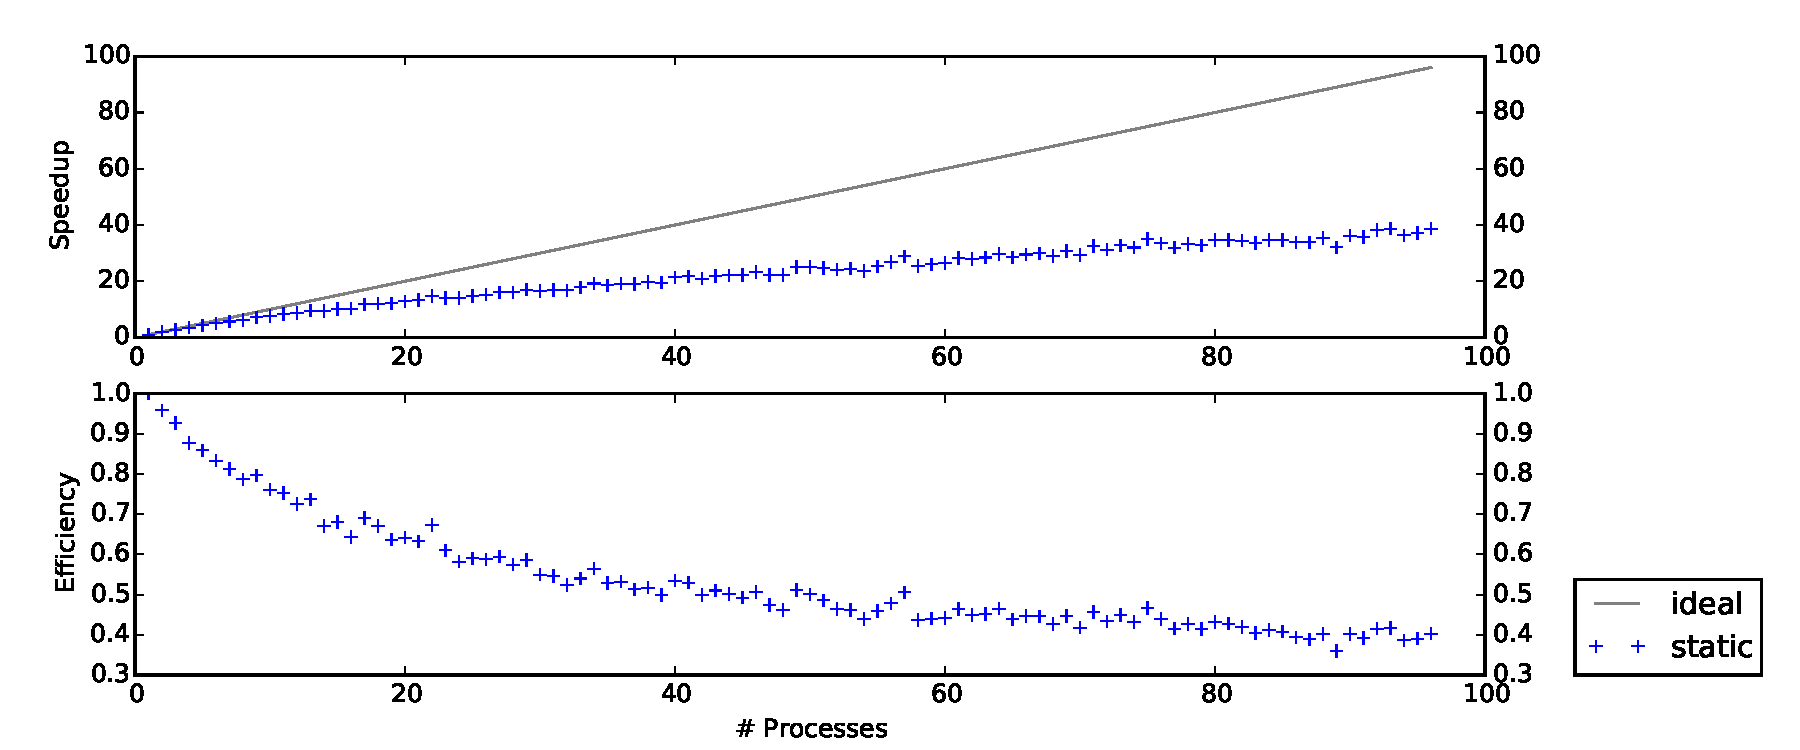
\includegraphics[width=\textwidth]
        {content/img/strong_scaling_time_static.pdf}
    \caption{Speedup bei statischer Lastverteilung}
    \label{fig:speedup_static}
\end{figure}

\begin{figure}
    \centering
    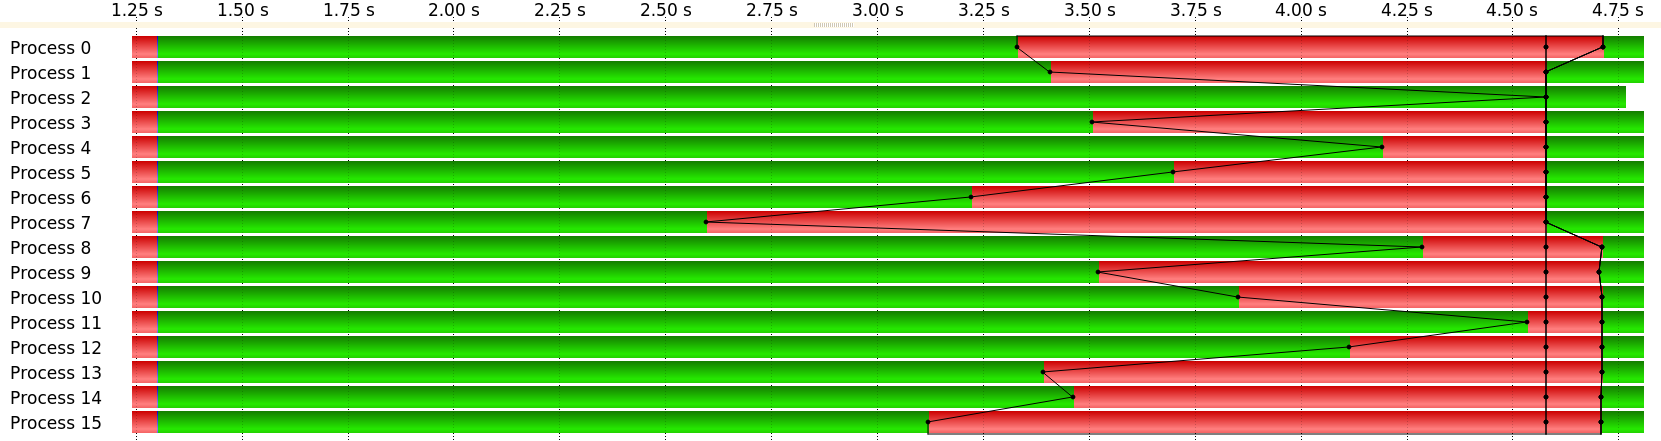
\includegraphics[width=\textwidth]
        {content/img/vampir_static.png}
        \caption{Prozess Timeline bei statischer Lastverteilung}
    \label{fig:vampir_static}
\end{figure}

In Abbildung \ref{fig:speedup_static} ist zu erkennen, dass die erreichte
Effizienz bei 96 Prozessen nur einen Wert von ungefähr \num{0,4} erreicht.
Dies liegt deutlich unter den erwarteten Werten. Eine Analyse mit Vampir \cite{vampir}
(Abbildung \ref{fig:vampir_static}) zeigt, dass eine Lastungleichheit zwischen den
Prozessen herrscht. Diese ist dadurch zu erklären, dass Spiele unterschiedlich
lange dauern. Die Länge eines Spiels wurde nach oben beschränkt: Nach 1024
Zügen wird es abgebrochen und die Punkte werden ausgezählt. Mindestens zwei
Züge sind notwendig, um ein Spiel zu beenden, da zweifaches Passen zum
Spielende führt.
Da die neuronalen Netze zufällig erstellt wurden und nach jeder Generation
zufällig verändert werden, ist es uns nicht möglich vorherzusagen, wie lange ein
Spiel zwischen zwei bestimmten Netzen dauernd wird.

\subsection{Dynamische Verteilung}

Gelöst wurde das oben beschriebene Problem der Lastungleichheit durch eine
dynamische Verteilung der Spiele auf die Prozesse.  Ein Masterprozess übernimmt
die Aufgabenverteilung, während die restlichen Workerprozesse, die Berechnungen
durchführen.  Zunächst wird ein Teil aller Spiele gleichmäßig auf alle
Workerprozesse verteilt. Ist ein Worker mit seinem Anteil fertig, schickt er
eine Anfrage an den Master. Falls noch Spiele zu berechnen sind, antwortet
dieser mit einem Auftrag zu bearbeitender Spiele, andernfalls wird mit einem
leeren Auftrag geantwortet.  Der Worker bearbeitet den Auftrag oder wartet
darauf, dass die anderen ebenfalls fertig werden.  Siehe Algorithmen
\ref{alg:master} und \ref{alg:worker}.

Dieser Ansatz wurde mit zwei Parametern untersucht. Zum
einen wurde der Anteil der initial verteilten Spiele (\emph{initial}) variiert,
zum anderen die Paketgröße (\emph{chunksize}). In der Legende der Diagramme
werden diese Konfigurationen in der Form $c-i$ dargestellt, wobei $i \in
\mathbb{N} \setminus \{0\}$ die Paketgröße und $i \in [0, 1]$ den Anteil
statisch verteilter Spiele angibt.

\begin{algorithm}
    \caption{Master}
    \label{alg:master}
    \begin{algorithmic}[1]
        \Require $initial, chunksize, n$ (number of games)
        \State $start \gets n \cdot initial$
        \While {$start < n$}
            \State $msg, worker \gets $\Call{Recv}{$anyone$}
            \State \Call{Send}{$worker, (start, \min(chunksize, n - start))$}
            \State $start \gets start + chunksize$
        \EndWhile
        \For {each process $p$}
            \State $msg, worker \gets $\Call{Recv}{$anyone$}
            \State \Call{Send}{$worker, (0, 0,$ "finished")}
        \EndFor
    \end{algorithmic}
\end{algorithm}
\begin{algorithm}
    \caption{Worker}
    \label{alg:worker}
    \begin{algorithmic}[1]
        \Require $initial, chunksize, n$ (number of games)
        \State $start, chunksize \gets \Call{partition}{n \cdot initial}$
        \While {$chunksize \neq 0$}
            \For {$g \in [start, start + chunksize)$}
                \State calculate game $\#g$
                \State count the ($wins$)
            \EndFor
            \State \Call{Send}{$master$, "request work"}
            \State $start, chunksize \gets $\Call{Recv}{$master$}
        \EndWhile
    \end{algorithmic}
\end{algorithm}

\subsubsection{Paketgröße}
Da die Anzahl an Anfragen mit sinkender Paketgröße steigt, wurde vermutet, dass
es einen Punkt gibt, ab dem die weitere Verkleinerung der Pakete für mehr
Overhead sorgt, als dass sie Zeit spart.
In Abbildung \ref{fig:speedup_chunksize} sind die Speedupkurven für Paketgrößen
von 1, 5 und 10 Spielen aufgezeichnet, während \SI{50}{\percent} der Spiele
gleichmäßig verteilt wurden. Es ist zu erkennen, dass bei der feinstmöglichen
Granularität von einem Spiel pro Paket, die erreichte Effizienz am größten ist.

\begin{figure}
    \centering
    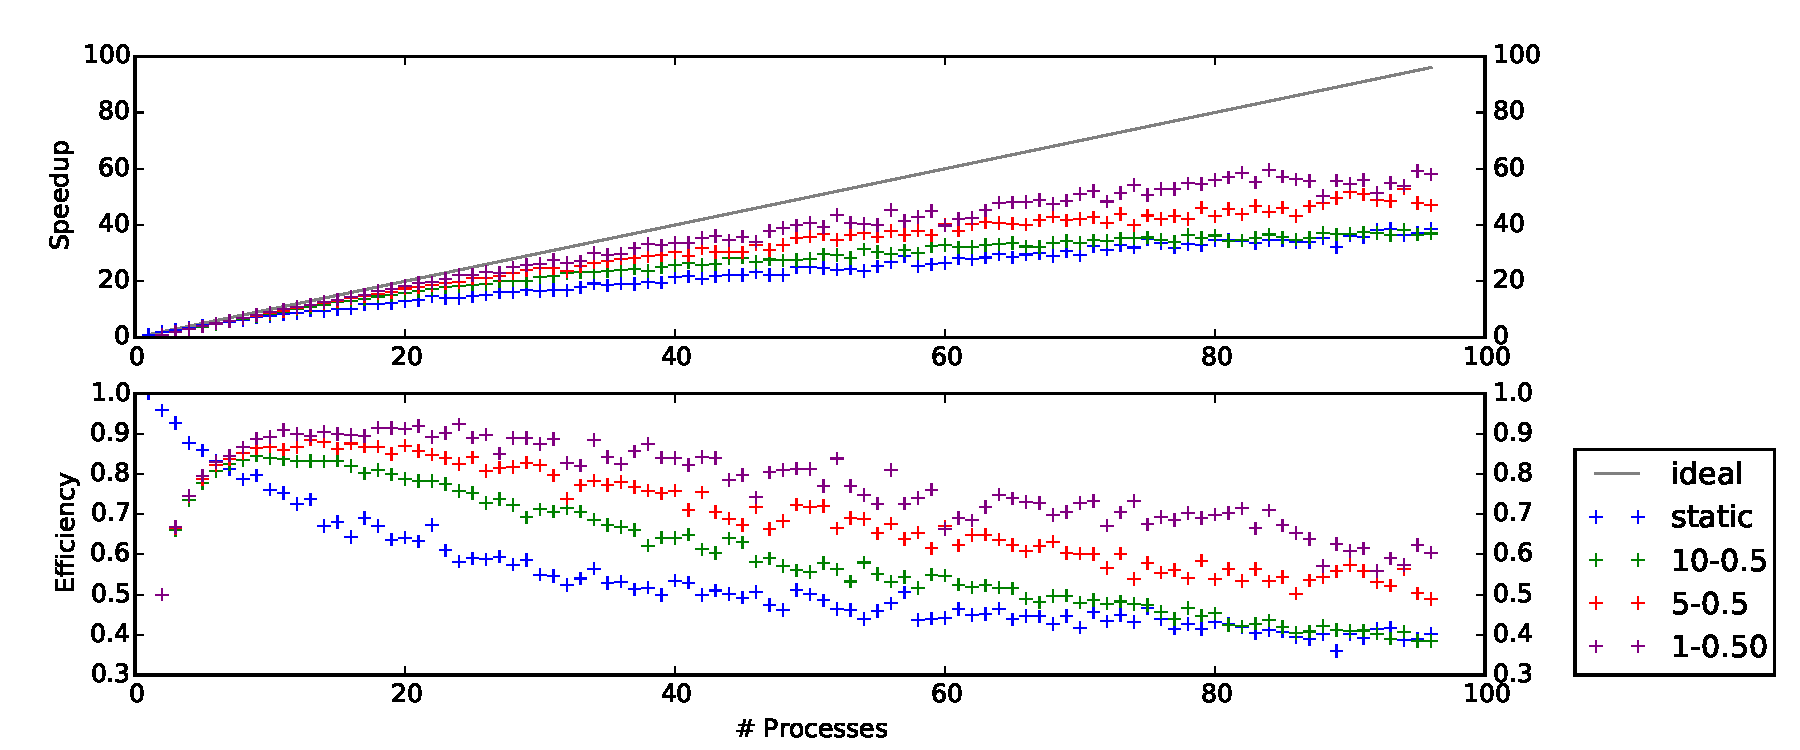
\includegraphics[width=\textwidth]
        {content/img/strong_scaling_time_chunksize.pdf}
    \caption{Vergleich von Paketgrößen}
    \label{fig:speedup_chunksize}
\end{figure}

\subsubsection{Anteil statischer Verteilung}
Der zweite Parameter gibt an, wie viele Spiele zu Beginn einer Generation
gleichmäßig auf die Worker aufgeteilt werden. Je größer der Anteil ist, desto
weniger muss über MPI kommuniziert werden. Abbildung \ref{fig:speedup_initial}
zeigt den Speedup für die initiale Verteilung von \SI{25}{\percent} bis
\SI{75}{\percent}. Je weniger statisch verteilt wurde, desto effizienter ist
die Parallelisierung. Aus Gründen der Übersichtlichkeit wurden nur drei
Konfigurationen im Diagramm aufgezeichnet. Durch Messungen wurde jedoch
festgestellt, dass initialen Verteilungen von maximal einem Drittel der Spiele
kein wesentlicher Unterschied mehr erreicht wurde.

\begin{figure}
    \centering
    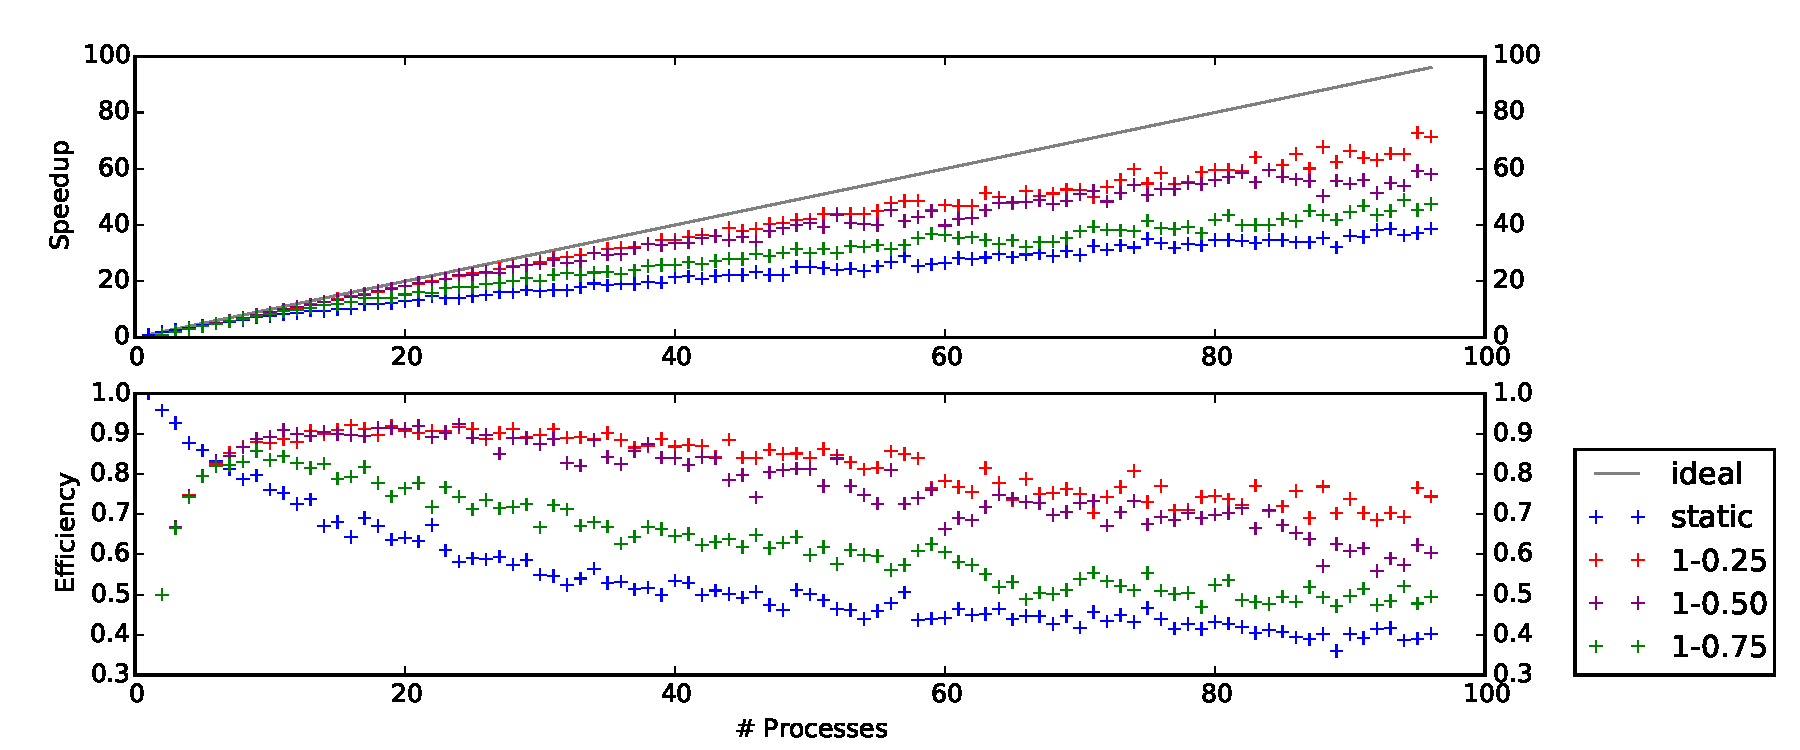
\includegraphics[width=\textwidth]
        {content/img/strong_scaling_time_initial.pdf}
    \caption{Vergleich von Anteilen der initial verteilten Spiele}
    \label{fig:speedup_initial}
\end{figure}

\subsubsection{Vergleich von dynamischer und statischer Verteilung}
Während der erste Ansatz beinahe ohne MPI-Kommunikation auskommt -- es werden
ausschließlich die Ergebnisse am Generationsende aufsummiert -- benötigt die
dynamische Verteilung pro verteiltem Paket zwei Punkt-zu-Punkt Übertragungen.
Zudem beteiligt sich der Masterprozess nicht an der Berechnung.  Dennoch kommt
es zu einem deutlichen Unterschied bezüglich Speedup und Effizienz (Abbildung
\ref{fig:speedup_final}): Mit ca. \SI{75}{\percent} Effizienz bei 96 Prozessen
erreicht die dynamische Verteilung ein wesentlich besseres Ergebnis als die
statische Aufteilung mit ca. \SI{40}{\percent}.

\begin{figure}
    \centering
    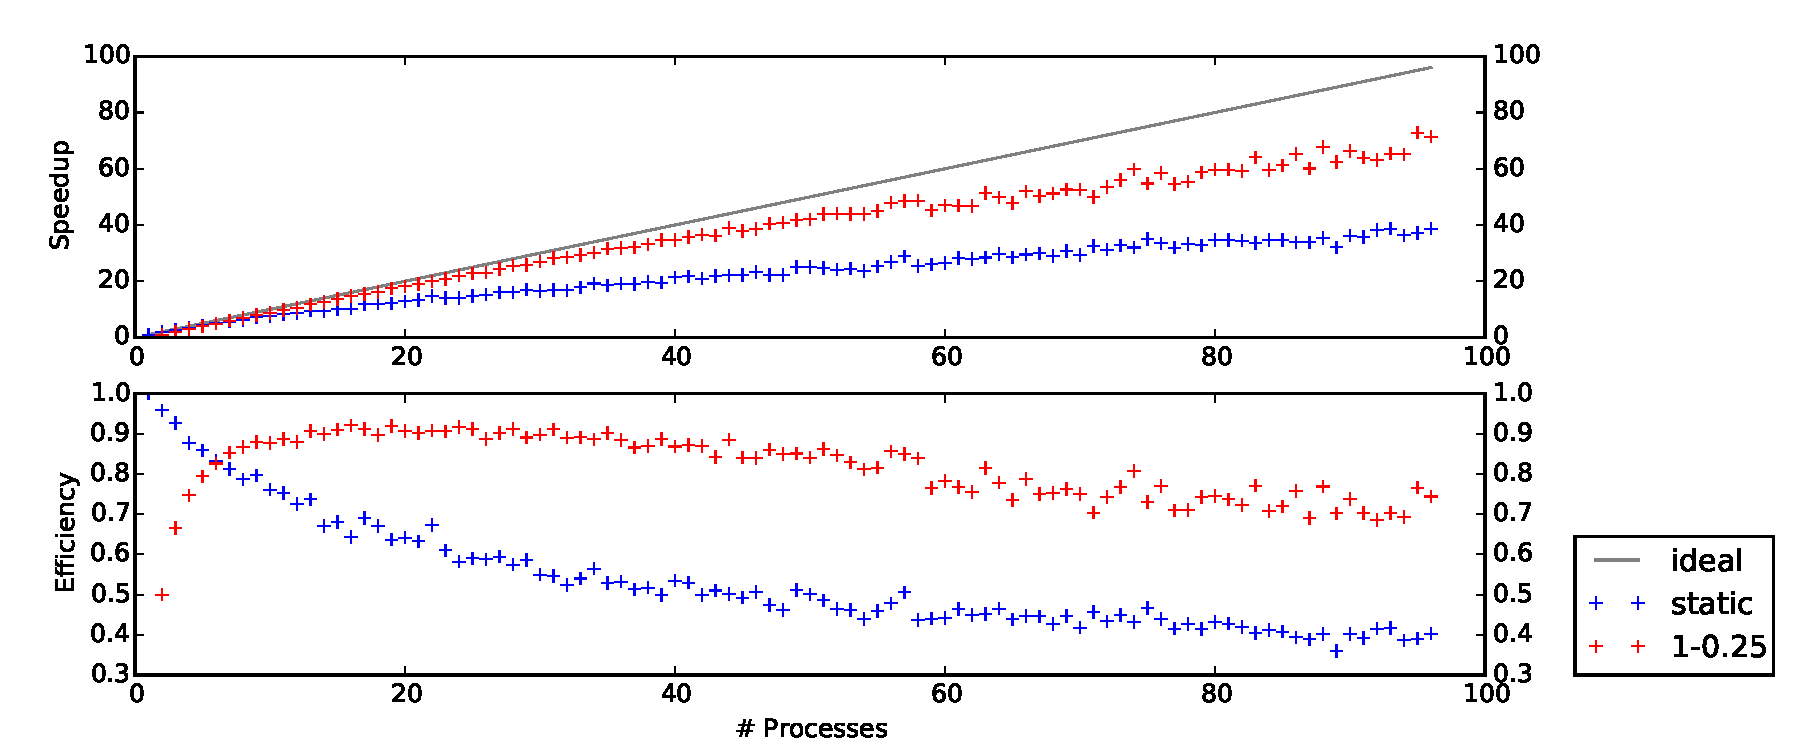
\includegraphics[width=\textwidth]
        {content/img/strong_scaling_time_final.pdf}
    \caption{Vergleich von dynamischer und statischer Lastverteilung}
    \label{fig:speedup_final}
\end{figure}

In Abbildung \ref{fig:vampir_dynamic} ist das Kommunikationsschema einer
Generation dargestellt. Der Masterprozess (Prozess 0) beantwortet ab
\SI{1,8}{\second} die eintreffenden Requests der Workerprozesse. Jeder
erkennbare Strich zwischen dem Master und einem Worker repräsentiert eine
Request und die dazugehörige Response.

\begin{figure}
    \centering
    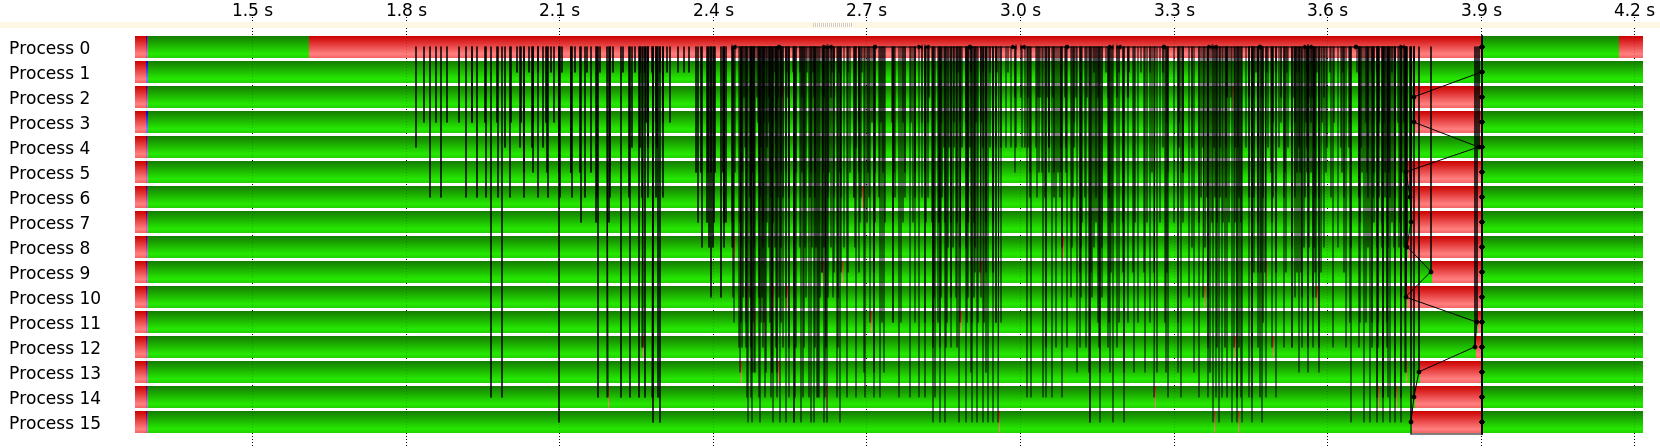
\includegraphics[width=\textwidth]
        {content/img/vampir_dynamic.png}
        \caption{Prozess Timeline bei dynamischer Lastverteilung}
    \label{fig:vampir_dynamic}
\end{figure}

Gut erkennbar sind die unterschiedlichen Längen der Spiele. Die grün
dargestellten Bereiche zwischen den MPI-Aufrufen auf den Balken der Worker
zeigen jeweils die Berechnung eines Spiels. Betrachtet man beispielsweise den
Prozess 15. Das erste vom Master zugeteilte Spiel wird ab \SI{2,1}{\second}
berechnet und braucht ungefähr \SI{0,2}{\second}. Anschließend bei ca.
\SI{2,3}{\second}, kommuniziert Prozess 15 zweimal kurz hintereinander mit dem
Master. In dem Intervall zwischen den beiden Anfragen wird ein weiteres Spiel
berechnet.

Die Antwortzeit bei den Anfragen ist im Vergleich zu der Zeit, welche für die
Berechnung eines Spiels aufgewendet wird, so gering, dass die Wartezeit für die
Worker vernachlässigbar gering bleibt. Auch die Wahrscheinlichkeit für
gleichzeitige Anfragen von mehreren Prozessen ist gering genug, so dass mit
synchronen Sende- und Empfangsinstruktionen gearbeitet werden kann.

Die Lastungleichheit ist weitestgehend behoben. Zum Ende der Generation muss
zwar noch gewartet werden, jedoch ist die Ausnutzung der verfügbaren Rechenzeit
im Vergleich zu der vorherigen Situation deutlich besser.

\subsection{Hybride Parallelisierung}
Zusätzlich zu obigem Parallelisierungsschema wurde hybride Parallelisierung mit
MPI und OpenMP ausprobiert.  Dabei wurde untersucht, wie sich die Aufteilung
der Schleifen in der Ausgabeberechnung der neuronalen Netzwerke auf
verschiedene Threads verhält.

In der Testkonfiguration wurde ein rechnender MPI-Prozess mit OpenMP-Threads
gestartet, so dass jeder Thread auf einem eigenen Prozessorkern läuft.  Mit
einem einzelnen Thread -- also sequentiell -- lag die Laufzeit deutlich über
der, der entsprechenden Variant ohne OpenMP.  Mit jedem zusätzlichen Thread
stieg die Laufzeit weiter an. Daher wurde dieser Ansatz wieder verworfen und
sich auf einen MPI-Prozess pro Prozessorkern beschränkt.

Zwar wird viel Rechenzeit in \texttt{nnnet\_calculate\_output} verbracht, aber
wir vermuten, dass Berechnung einer einzelnen Ausgabe schnell genug ist, so
dass der Overhead beim Erstellen und Zerstören der Threads gegenüber der
eingesparten Rechenzeit deutlich überwiegt. Da bei jedem Zug eine Ausgabe
berechnet wird resultieren viele und lange Spiele einer anteilig hohen
Benutzung dieses Codeabschnitts.
